\section{Rust}
\label{Rust}
\lstset{language=rust}

\textit{Rust} ist eine kompilierte Programmiersprache, welche auf mehrereren
Programmierparadigmen aufbaut. Die Sprache krönt sich damit, dass
sie extrem schnelle und sichere Binärprogramme erzeugt. \cite{rustlangbook1}
Der gesamte Quellcode vom gesamten Rust-Ökosystem ist quelloffen. Rust besitzt keinen Garbage-Collector,
Arbeitsspeicher wird mithilfe des Ownership-Models verwaltet.

\subsection{Warum Rust?}
Wir haben uns beim Komponent \textit{Shulker-Core}, also bei der Programmierung
des Touchdisplays und der Hardwareschaltung, sowie der Speicherung
von Daten, für Rust entschieden. Diese Entscheidung trafen wir primär
aus fünf Gründen:

\begin{itemize}
    \item Das Ownership-Model und die Einfachkeit von nebenläufiger Programmierung in Rust zwingt uns, vor allem im Bereich vom Touchdisplay, zu einer korrekten Lösung und weniger Fehlern
    \item Vorkenntnisse in \textit{Rust} und dem UI-Toolkit \textit{Slint} erleichtern uns das Arbeiten
    \item Die hohe Performance des Endprodukts minimiert die Hardwareauslastung
    \item Die Einfachkeit der Kompilierung macht es dem Nutzer leichter
    \item Da Rust eine Systemprogrammiersprache ist, ermöglicht es hardwarenahe Programmierung trotz hoher Abstraktionen
\end{itemize}

\subsection{Geschichte von Rust}
Rust enstand im Jahr 2006 als Hobbyprojekt von Graydon Hoare, einem Angestellten
bei Mozilla. Im Jahr 2009 begann Mozilla das Projekt zu unterstützen. Die erste
offiziell stabile Version (Version 1.0) wurde im Jahr 2015, also ganze neun Jahre danach, veröffentlicht.
Im Jahr 2020 wurden 250 Angestellte von Mozilla entlassen.  Ein großer
Teil des Rust Teams wurde damit entlassen. Das schien eine Bedrohung für
die Programmiersprache zu sein. Glücklicherweise wurde im darauffolgenden Jahr die
\textit{Rust Foundation} von den Firmen \textit{AWS, Google, Huawei, Microsoft und Mozilla} gegründet.
Rust wurde in der \textit{Stackoverflow Developer Survey}, einer großen Umfrage
für Programmierer, 2016, 2017, 2018, 2019, 2020 und 2021 zur am meisten geliebten Programmiersprache
ernannt. Ob das im Jahr 2022 so der Fall bleibt, wird sich zeigen.


\subsection{Programmierparadigmen}
Rust bietet verschiedenste Möglichkeiten, seinen Code zu gestalten. Unter
anderem borgt sich die Sprache Ideen von der funktionalen und objektorientierten
Programmierung. Auch das nebenläufige Programmieren, unter Rust-Usern als
\textit{Fearless Concurrency} bekannt, ist möglich. Man programmiert in Rust
primär imperativ, deklaratives Programmieren ist trotzdem auch ein wichtiger
Teil der Programmiersprache.

\subsection{Ownership-Model}
Jedes auf auf einem herkömmlichen Computer ausgeführte Programm muss den eigenen Arbeitsspeicher selbst verwalten.
Der Arbeitsspeicher wird in Stack und Heap eingeteilt. \cite{rustlangbookownership1}

Der Stack funktioniert auf dem \textit{First-In-First-Out}-Prinzip. Man kann das Prinzip mit einem Stapel Teller vergleichen.
Will man dem Tellerstapel (also dem Teller-Stack) einen Teller hinzufügen, ist es einfacher,
den Teller auf den Stapel dazu zulegen. Will man einen Teller wegnehmen, ist das am einfachsten indem man den obersten Teller wegnimmt.
Auf dem Stack kann man also nur einen Wert auf die oberste Stelle abspeichern und eben genau den obersten, also den als letztes hinzugefügten
Wert entfernen. Alle auf dem Stack speicherbaren Daten müssen eine bekannte und konstante Größe aufweisen, also eine genau definierte Anzahl
an Bits einnehmen. Zur Speicherung von Daten mit einer zur Kompilierzeit unbekannten oder variablen Größe muss der Heap verwendet werden.

Auf dem Heap herrscht nur minimale Ordnung. Will man Daten auf dem Heap ablegen, muss sich das Computerprogramm einen Teil des Heaps
reservieren. Um erst mal einen Teil des Heaps verwenden zu können, muss ein \textit{memory allocator} (ein Teil des Programms) einen nicht
verwendeten und groß genugen Teilbereich des Heaps finden und als benutzt markieren. Der memory allocator liefert im Anschluss einen Pointer zurück,
also eine Speicheraddresse, welche auf den Beginn des neu belegten Heapspeicherteils zeigt. Den Pointer kann man dann auf den Stack speichern, da eine
Speicheraddresse eine fixe Anzahl an Bits einnimmt. Wichtig: Der Heap erfordert das Freigeben der reservierten Speicherteile, wenn sie nicht
mehr in Gebrauch sind. Wird der Speicher nicht befreit, kann es zu Problemen kommen. Zum Beispiel könnte der Arbeitsspeicher bei längerer
Ausführung des Programms voll laufen, da immer mehr und mehr Teile des Heaps als benutzt markiert werden.

Bei Sprachen wie \textit{C} und teilweise auch \textit{C++} liegt die Verantwortung des Heaps in den Händen der Programmierer. Der Programmierer
muss manuell Heapspeicher anlegen und befreien. Bugs haben so ein leichtes Spiel, da jeder Mensch Fehler macht. Viele höhere Programmiersprachen setzten
deshalb zur Vereinfachung und Fehlervermeidung auf einen \textit{Garbage Collector}. Der Garbage Collector scannt regelmäßig nach nicht mehr
gebrauchten Speicher. Findet er nicht mehr gebrauchten Speicher, markiert er diesen Teil des Arbeitsspeichers als ungenutzt und ermöglicht so 
das Wiederverwenden dieses Speicherabschnitts. Ein Garbage Collector hat aber einen großen Nachteil: Er ist ineffizient.

Um dem Problem der Ineffizienz zu entgehen verwendet Rust das \textit{Ownership-Model}. Das Model besteht
aus drei Regeln, welche zur \textit{compile time}, also während des Kompilierprozesses, im Quellcode validiert werden. Erfüllt der Rustcode nicht
alle diese Regeln weist der Compiler auf den Fehler hin und bricht die Kompilation ab. Somit wird das Auftreten von Fehlern in der Speicherverwaltung
vollständig behoben. Laut \textit{Google} sind ungefähr 70\% aller Sicherheitsbugs in \textit{Google Chrome} mit inkorrekter Speicherverwaltung verbunden. \cite{googlechrome70}
Das Ownership-Model allein würde einen Großteil dieser Sicherheitsbugs ausschließen.

Die drei Ownership-Regeln lauten:

\begin{itemize}
    \item Jeder Wert ist einer Variable zugeteilt, welche man den \textit{Owner} (Besitzer) nennt
    \item Es kann immer nur einen Owner geben
    \item Wenn der Owner out-of-scope fällt, wird der zugewiesene Wert gedropped (der Speicher wird freigegeben)
\end{itemize}
\cite{rustlangbookownership2}

\subsection{Scope von Variablen}
Der Scope einer Variable ist der Bereich im Quellcode, in dem eine Variable gültig ist. Ein kleines Beispiel:

\begin{lstlisting}
    let x: i32 = 10;
\end{lstlisting}

Hier wird eine Ganzzahl (ein Integer), die 32 Bit an Information einnimmt, angelegt. Die Variable \textit{x} hat also den Wert \textit{10} vom Typ \textit{i32};
Aus dem Beispiel ist der \textit{Scope} von x aber nicht ablesbar. Eine Erweiterung mit Scope:

\begin{lstlisting}
    {
        let x: i32 = 10;
    }
\end{lstlisting}

Der Scope von x liegt hier innerhalb der geschwungenen Klammern. Ein Zugreifen auf x außerhalb des Scopes ist nicht möglich. x existiert also nur
zwischen den Klammern. Um genauer zu sein: x existiert von der Deklaration bis hin zum Ende des Scopes:
\begin{lstlisting}
    println!("{}", x); // <- Fehler
    {
        println!("{}", x); // <- Fehler
        let x: i32 = 10;
        println!("{}", x); // <- Funktional
    }
    println!("{}", x); // <- Fehler
\end{lstlisting}

Dieses Verhalten ist in vielen bekannten Programmiersprachen identisch, also was ist nun das \textbf{besondere} an Rust? Da ein 32 Bit Integer
eine zur Kompilierzeit bekannte und konstante Größe hat, kann x einfach auf dem Stack gespeichert werden. Rusts Vorteile werden beim Umgang mit
auf dem Heap gespeicherten Daten erst richtig ersichtlich. Als Veranschaulichung werden wir den \textit{String}-Typen verwenden, da er eine
variable Größe hat:
\begin{lstlisting}
    {
        let s1 = String::from("Shulker");
        let s2 = String::from("HTL-Anichstrasse");
    }
\end{lstlisting}

Da der String \textit{s2} mehr Zeichen als der String \textit{s1} hat, braucht \textit{s2} auch mehr Speicherplatz. Strings können auch zur Laufzeit
verändert werden. Man könnte zum Beispiel dem \textit{Shulker}-String eine zufällige Zahl hinzufügen. Das verändert natürlich den Speicherbedarf zur
Laufzeit. Somit ist klar, dass Strings auf dem Heap abgelegt werden müssen.

\subsection{Der Drop Trait}
Wie es in der letzten Regel des Ownership-Models beschrieben wird, werden Variablen die out-of-scope fallen gedropped. Gedropped bedeutet, dass Rust
eine Funktion namens \textit{drop} ausführt, welche den Speicher der out-of-scope gefallenen Variable befreit. Die \textit{drop}-Funktion wurde in
unserem Fall von den Entwicklern vom String-Typ implementiert. Rust regelt also, wann eine Variable gedropped werden kann und sollte. Der Programmierer
muss sich keine Gedanken darum machen, den Heap-Speicher zu befreien.

\subsection{Immer nur ein Owner}
Eine Regel des Ownership-Models besagt, dass ein Wert immer nur einen Owner zugeteilt sein darf. Welche Auswirkungen das auf unseren Code hat, kann anhand
von wenigen einfachen Beispielen veranschaulicht werden:
\begin{lstlisting}
    let a = 10;
    let b = a;
\end{lstlisting}
Im obigen Beispiel ist die Variable \textit{a} der Owner von den Daten mit dem Wert \textit{10}. In der zweiten Zeile sollte dann die Variable \textit{b}
der Owner vom Wert in der Variable \textit{a} werden, oder? Wäre das der Fall, würde die zweite Regel des Ownership-Models gebrochen werden. Es würde zwei
Owner von dem gleichen Speicherort zur gleichen Zeit geben, \textit{a} und \textit{b}.

\subsubsection{Der Copy Trait}
Da der Wert 10 einfach kopiert werden kann, wird er auch kopiert. \textit{b} wird also nicht der Owner von den gleichen Daten wie \textit{a}, sondern
von einer Kopie der Daten in \textit{a}. Das obige Beispiel wäre also equivalent zu:
\begin{lstlisting}
    let a = 10;
    let b = 10;
\end{lstlisting}
In Rust nennt man dieses Verfahren des einfachen Kopierens \textit{copy}. Wird ein Wert kopiert, so ruft Rust die Funktion \textit{copy} auf. Das
ist aber nur möglich, wenn der zu kopierende Wert den Copy-Trait besitzt. Grundsätzlich müssen Daten nur eine Vorraussetzung erfüllen, um den
Copy Trait besitzen zu dürfen: Der Wert muss vollständig kopierbar sein.

\subsubsection{Das Problem mit Copy}
Das obige Beispiel hat auf dem Stack gespeicherte, einfach zu kopierende Werte verwendet. Im folgenden Beispiel werden jetzt auf dem Heap gespeicherte,
nicht ganz so einfach zu kopierende Daten verwendet. Strings um genau zu sein:
\begin{lstlisting}
    let a = String::from("Shulker");
    let b = a;
\end{lstlisting}
Man könnte jetzt denken, dass der String \textit{a} einfach mittels copy zu \textit{b} kopiert wird. Das würde aber die Ownership-Regel brechen, dass
es nur einen Owner zur gleichen Zeit geben darf. Auf den ersten Blick wird dieser Umstand nicht ganz klar. Dafür muss man sich anschauen, wie Strings
in Rust aufgebaut sind:
\begin{figure}[H]
    \begin{center}
        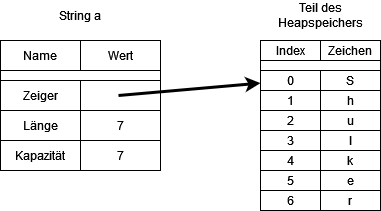
\includegraphics[width=0.55\textwidth]{images/rust/string_repr.png}
        \caption{Veranschaulichung eines Rust-Strings}
    \end{center}
\end{figure}
Würde man den Copy-Trait nutzen, also einfach Bit für Bit kopieren, würde folgende Situation resultieren:
\begin{figure}[H]
    \begin{center}
        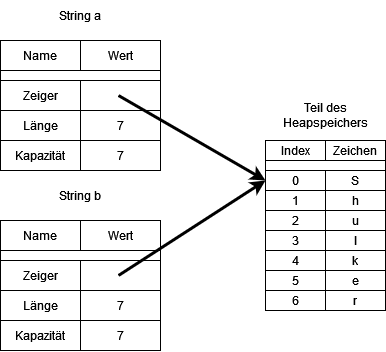
\includegraphics[width=0.55\textwidth]{images/rust/string_copy_repr.png}
        \caption{Bild zur Veranschaulichung eines kopierten Rust-Strings}
    \end{center}
\end{figure}
\subsection{move}
Wie man sieht, würden beide Variablen auf die selben Daten zeigen. Es würde also wieder zwei Owner zur gleichen Zeit geben. Die Regeln des Ownerships würden
nicht eingehalten werden. Um dieses Problem zu umgehen, wird die Variable a als nicht mehr gültig angesehen. Wichtig: a wird nicht gedropped, sonst
würde b auf nicht existente Daten zeigen. Das nennt man \textit{move}:
\begin{lstlisting}
    let a = String::from("Shulker");
    let b = a;
    println!("{}", a); // <- Fehler
    println!("{}", b); // <- funktional, a wurde in b "gemoved"
\end{lstlisting}
\textit{Shallow Copy} ist eine wichtige Begrifflichkeit in vielen Sprachen. \textit{Shallow copy} ist dem Verhalten von \textit{move} sehr ähnlich. Einen
großer Unterschied gibt es jedoch: Die Invalidierung der ersteren Variable. Dieses Verhalten existiert so nur bei \textit{move}.

\subsection{clone}
Will man also korrekt den String \textit{a} kopieren, verwendet man \textit{clone}. Clone ist im Grunde genommen das gleiche wie eine \textit{deep copy}.
Es werden nicht nur die Daten auf dem Stack kopiert, sondern auch die auf dem Heap:
\begin{lstlisting}
    let a = String::from("Shulker");
    let b = a.clone();
    println!("{}", a); // <- funktional
    println!("{}", b); // <- funktional
\end{lstlisting}
\begin{figure}[H]
    \begin{center}
        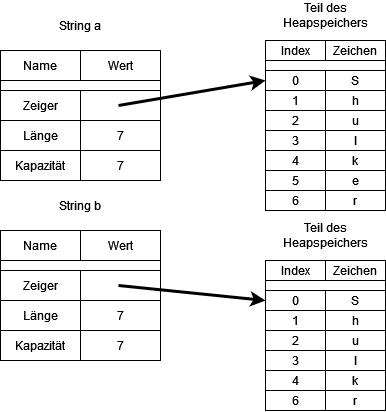
\includegraphics[width=0.5\textwidth]{images/rust/string_clone_repr.png}
        \caption{Bild zur Veranschaulichung eines geklonten Rust-Strings}
    \end{center}
\end{figure}

\subsection{Ownership und Funktionen}
Eine Funktion ist ein eigener Scope. Daraus resultiert sich, dass Variablen am Ende einer Funktion out-of-scope fallen und gedropped werden müssen:
\begin{lstlisting}
    fn sag_hallo(name: String) {
        println!("Hallo {}", name);
    } // <- name wird gedropped

    fn main() {
        let mein_name = String::from("Alexander");
        sag_hallo(mein_name);
    }
\end{lstlisting}
Es gibt hierbei ein Problem. Man kann die Variable \textit{mein\_name} nicht wiederverwenden:
\begin{lstlisting}
    fn sag_hallo(name: String) {
        println!("Hallo {}", name);
    } // <- name wird gedropped

    fn main() {
        let mein_name = String::from("Alexander");
        sag_hallo(mein_name);
        println!("Bis spaeter {}", mein_name);
        // ^ Fehler, da mein_name gedropped wurde
    }
\end{lstlisting}
Anzumerken ist hierbei jedoch, dass Variablen welche den copy trait besitzen, also nicht gemoved werden müssen, einfach kopiert werden. Das
Problem gibt es also nur, wenn man komplexere Datentypen einer Funktion als Parameter übergeben will.

Es gibt grundsätzlich zwei Lösungswege:

Man könnte die übergebene Variable wieder zurückgeben:
\begin{lstlisting}
    fn sag_hallo(name: String) -> String {
        println!("Hallo {}", name);
        return name; 
    //  ^ name wird zurueckgegeben und nicht gedropped
    }

    fn main() {
        let mein_name = String::from("Alexander");
        let mein_name = sag_hallo(mein_name);
    //  ^ Rueckgabewert wieder in mein_name uebergeben
        println!("Bis spaeter {}", mein_name);
    }
\end{lstlisting}

Der elegantere Lösungsweg macht sich Referenzen zu nutze. Referenzen sind in Rust so ähnlich wie Pointer, nur dass Referenzen
garantieren, dass die Daten auf die gezeigt wird noch valide sind. Referenzen werden durch das Zeichen \& gekennzeichnet. Die Lösung
ist somit um einiges angenehmer:
\begin{lstlisting}
    fn sag_hallo(name: &String) {
        println!("Hallo {}", name);
    } // Referenz wird gedropped, Wert aber nicht

    fn main() {
        let mein_name = String::from("Alexander");
        sag_hallo(&mein_name);
        println!("Bis spaeter {}", mein_name); // funktioniert
    }
\end{lstlisting}

Referenzen sind ein riesiger Bestandteil von Rust und somit auch des Shulker-Quellcodes.

\subsection{Mutabilität und mutable Referenzen}
Alle Variablen in Rust sind grundsätzlich unveränderbar. Um den Wert einer Variable dennoch zu verändern,
muss diese als \textit{mutable} gekennzeichnet werden. Dafür gibt es das \textit{mut} Keyword:
\begin{lstlisting}
    let mut a = 10;
\end{lstlisting}
Will man den Wert durch eine Referenz verändern, muss die Referenz und der Owner als veränderbar gekennzeichnet werden:
\begin{lstlisting}
    fn veraendern(name: &mut String) {
        name.push('a');
    } // Referenz wird gedropped, Veraenderung bleibt

    fn main() {
        let mut mein_name = String::from("Alexander");
    //  ^ Achtung: mein_name muss mutable sein
        veraendern(&mut mein_name);
    // mein_name ist nun "Alexandera"
    }
\end{lstlisting}
Zu beachten ist:
\begin{itemize}
    \item Es kann entweder eine mutable Referenz oder unendlich viele immutable Referenzen zur gleichen Zeit geben
    \item Jede Referenz muss valid sein
    \item Referenzen dürfen nicht länger als der Owner leben
\end{itemize}
Um den Quellcode von Shulker-Core nachvollziehen zu können, ist es essentiell, die bereits genannten Konzepte zu verstehen.

\subsection{Der Cargo Packagemanager}
\textit{Cargo} ist Rusts Packagemanager. Cargo übernimmt das Herunterladen von Packages (Codebibliotheken), das Kompilieren von Quellcode und weiteres.
Er ist der Hauptbestandteil des Rust Ökosystems. Cargo lässt sich leicht mit \textit{Rustup} installieren (Rusts offiziellem Installer). Shulker-Core macht
starken Gebrauch von Cargo. Die Installation und Nutzung ist besonders simpel, was das Aufsetzen des Raspberry Pis vereinfacht.

\subsection{Crates.io}
\textit{crates.io} ist die offizielle Sammlung von Rust-Packages, auch \textit{crates} genannt. Cargo greift standardmäßig auf diese 
Sammlung zu, um benötigte Packages zu installieren und in die Kompilierte Datei einzubinden.